\chapter{Introduction}

Morphological change has been demonstrated to accelerate evolution of
robust behaviour in one instance. However, it is unclear how or why
this happens. This project evolves a robot with varying degrees of
conservation between the earlier and later forms to help answer the
question, under what conditions does morphological change accelerate
evolution?  Introduction Bongard showed the evolution of light
following behaviour was accelerated for robots that grew from a
leg-less anguilliform to a legged hexapod when compared to evolving a
hexapod with no morphological change [1]. This project is a critical
replication of that experiment.


\begin{comment}
  mention Minimal Simulation guy
  
  conventions bold denotes a vector
  hat means its a unit vector
  
\end{comment}

\chapter{Method}

This experiment uses a two-dimensional, aquatic-like environment to
test what kinds of morphological changes may accelerate evolution. The
morphological forms---inspired by frog metamorphosis---have been
selected such that the conservation of the infant form to the adult
form may be varied. Figure~\ref{morphology} shows the two principle
forms which may be parametrically varied by two variables $l_t, l_f
\in [0, 1]$ tail length and foot length respectively.  The full range
of morphological change will be described in detail in
section~\ref{morph-change}.  In the inspiring case, the individual
begins as a ``tadpole'' bearing only a tail. It transforms into a
``frog'' with four limbs. Its task is to swim to a target.

%\begin{wrapfigure}{r}{0.5\textwidth}
\begin{figure}[h]
  \centering
  \figtitle{Body Plans} 
  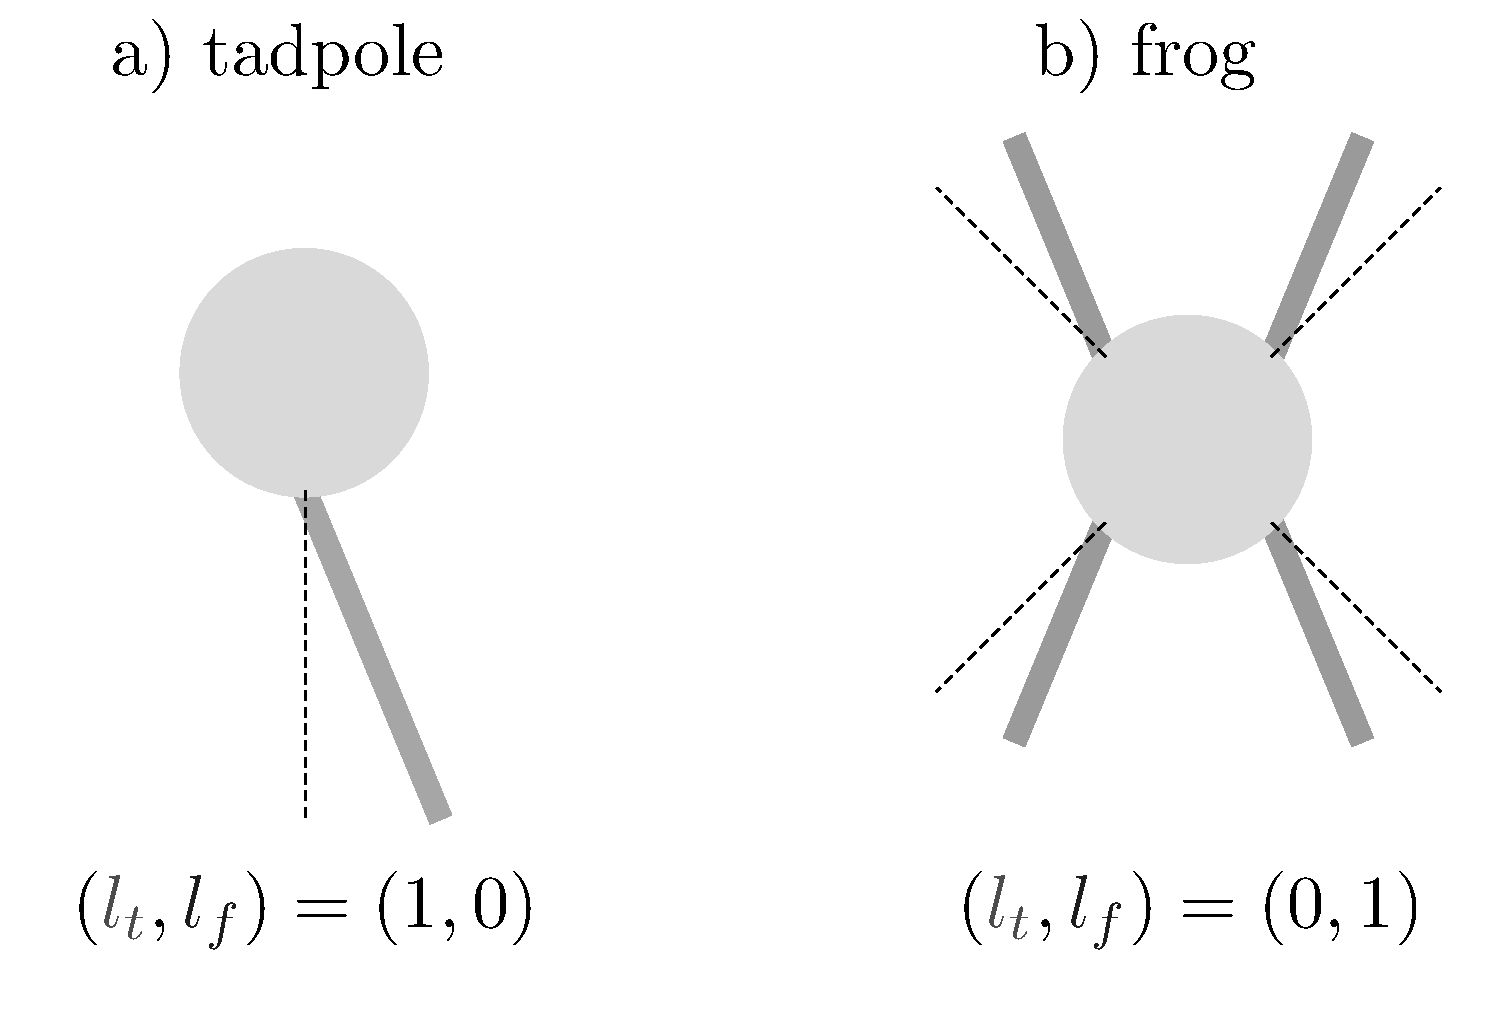
\includegraphics[scale=0.4]{fig/forms-gs.pdf} 
  \vspace{-30pt}
  \caption[Body plans]{\label{morphology}Body plans parameterised by
    tail length $l_t$ and foot length $l_f$. a) represents the infant
    ``tadpole'' form, and b) represents the adult ``frog'' form. }
\end{figure}
%\end{wrapfigure}

\section{Physics Model}

This experiment uses the following physical model to simulate an
individual in an two-dimensional aquatic environment.  The aim of the
simulation is to provide a water-like environment, but it is not
intended to provide a realistic environment such that a controller
evolved in simulation could be easily transferred to a real robot.  It
is thought, however, that applying the same method with a real robot
would produce comparable results.

The virtual robot is composed of six rigid bodies: one central body,
one tail segment, and four feet segments.  The tail and feet are
connected to the central body by pinwheel joints.  Eight configuration
variables $\{q_1, q_2, \ldots, q_8\}$ describe the body as shown in
Figure~\ref{confvars}.  The position of the body is denoted by the
vector $(q_1, q_2)$.  The angle of the central body measured
counter-clockwise to the $\bf \hat j$ axis denoted by $q_3$.  The
angle of the tail and four feet are denoted by $q_4, \ldots, q_8$,
respectively.  Eight corresponding motion variables $\{u_1, u_2,
\ldots, u_8\}$ describe the generalised speeds of the body $u_i =
\frac{d q_i}{d t}$.

\begin{figure}  
  \centering
  \figtitle{Diagram of Configuration Variables} 
  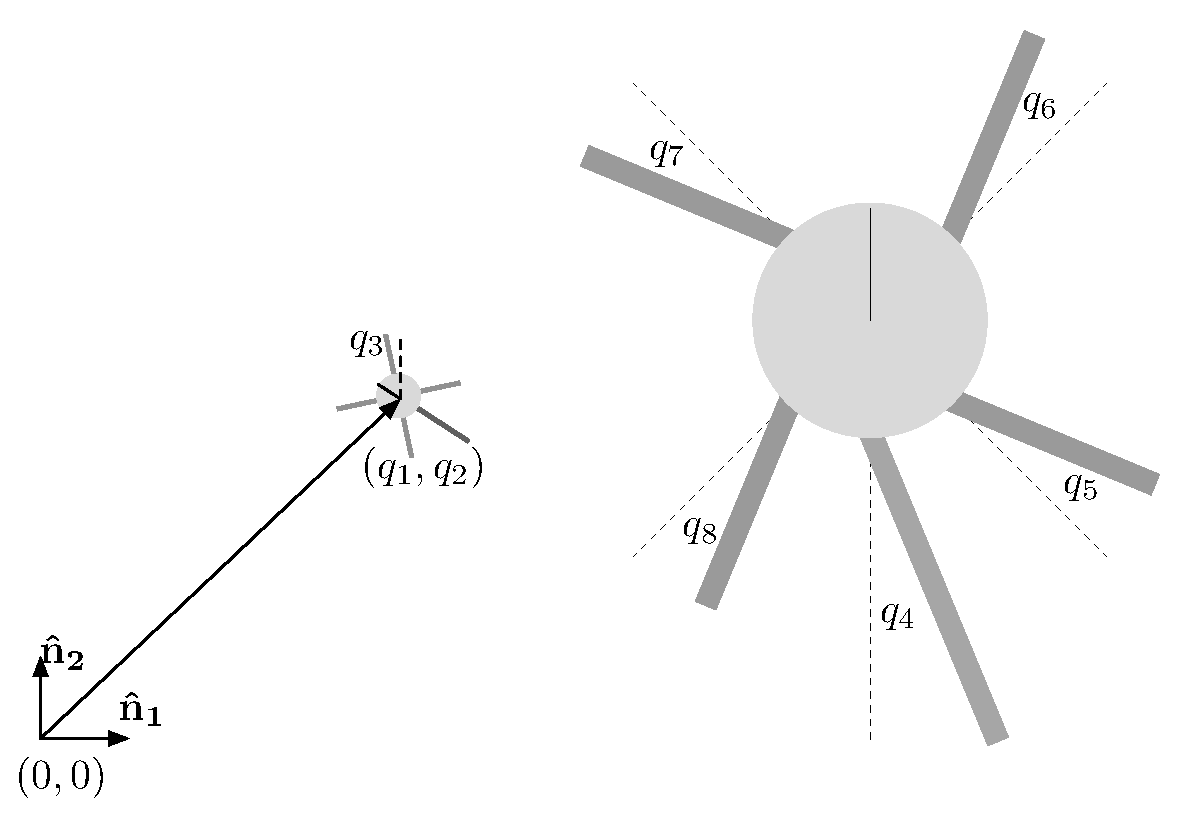
\includegraphics[scale=0.6]{fig/confvars-gs.pdf} 
  \caption[Diagram of configuration variables]{\label{confvars}Diagram
    of the configuration variables $\{q_1, q_2, \ldots, q_8\}$ that
    fully describe the physical state of the body at time $t$}
\end{figure}

\section{Forces}

For each limb a drag force $\bv F_D$ opposes its direction of motion
which are given by Equation~\ref{drag-force-eq} where $\rho$ is the
density of the fluid, $c_d$ is the drag coefficient, $l$ is the length
of the limb, $w$ is the width of the limb, $\bhv n$ is the normal of
the limb, $\bv v_b$ is the velocity of the center of mass of the limb,
$\bv v_c$ is the velocity of the current, $\bv v$ is the relative
velocity of the limb with respect to the current, $A$ is the reference
area---an orthographic projection of the limb shape on a plane
perpendicular to the direction of motion.  Figure~\ref{drag-force}
shows these values for a limb.  The shape of the limb is taken to be a
rod of length $l$, width $w$, and depth $d$.  However, for the
purposes of computing the drag force, the width of the limb $w$ is set
to zero since $w \ll l$ and the force it might contribute is not
considered significant.

\begin{eqnarray}
  A &=& l\,d~ |\bhv v \cdot \bhv n| + l\, w~|\bhv v \times \bhv n|\\
  w &=& 0 \\
  \bv v &=& \bv v_b - \bv v_c \\
  \bv F_D &=& -\frac{1}{2} \rho\,c_d~||\bv v||^2\,A~\bhv v \\
  \bv F_D &=& -\frac{1}{2} \rho\, c_d~ l\,d~|\bv v \cdot \bhv n|\bv v \label{drag-force-eq} 
\end{eqnarray}


\begin{figure}[h]  
  \centering
  \figtitle{Diagram of Drag Force} 
  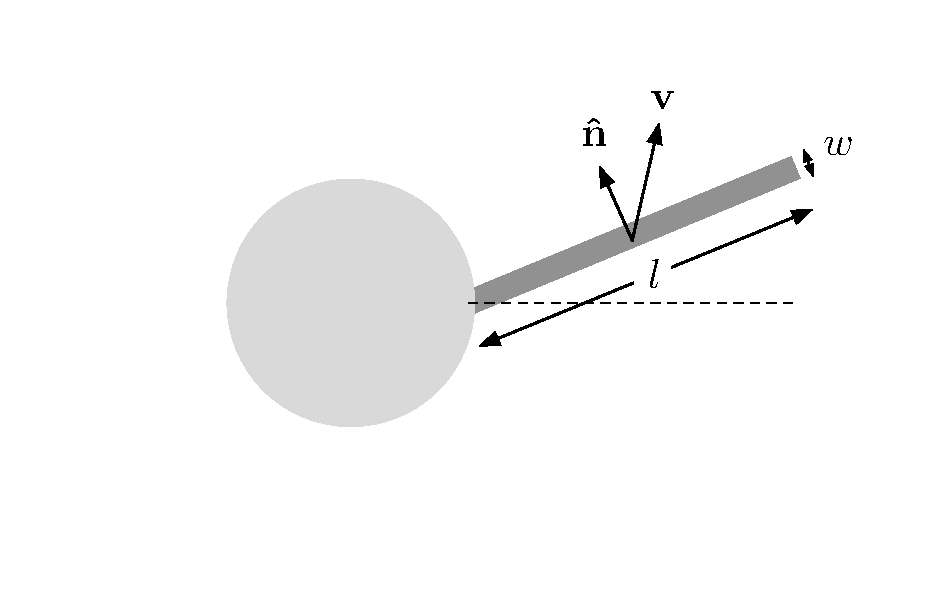
\includegraphics[scale=0.7]{fig/drag-force.pdf} 
  \vspace{-45pt}
  \caption[Diagram of drag force]{\label{drag-force}For each limb the
    length $l$, width $w$, depth $d$ (not shown), velocity of limb
    $\bv v_b $, velocity of current $\bv v_c$,, normal vector $\bhv n$
    determine its drag force $\bv F_D$.}
\end{figure}

In addition, a drag force and drag torque is exerted on the central
body.  The full equations of motion are given in the
Appendix~\ref{app:physeqns}.

\subsection{Collisions}

Interbody collisions are permitted, so limbs may freely move through
one another.\footnote{This is not thought objectionable because one
  can imagine constructing a robot with limbs arranged on planes such
  that they could pass each other unobstructed.}  However, the limbs
are constrained to not penetrate the central body.  When the angle of
a limb reaches $|q| = \frac{\pi}{2}$, a torque $T_c(q)$ is applied to
oppose further motion, shown in Equation~\ref{limb-bounded}.

\begin{eqnarray}
  T_c(q_{i}) &=& T_{max}~\bound(q_{i}, (\frac{- \pi}{2}, \frac{\pi}{2})) \text{ for } i \in [4,8] \label{limb-bounded} \\
  \bound(x, (a,b)) &=& \begin{cases}
    -1 & a \ge x \wedge b > x \\ 
    1 & a < x \wedge b \le x \\
    0 & \text{otherwise}
  \end{cases}
\end{eqnarray}


\section{Controller}

The controller used for the robot is a Continuous Time Recurrent
Neural Network (CTRNN).  The dynamics of a neuron $y_i$ is given by
Equation~\ref{ctrnn-eq} with time constant $\tau_i \in [0.1, 100]$,
weights $w_{ji} \in [-4, 4]$, bias $\theta_i \in [-2, 2]$, sensors
$s_j \in \R $, and sensor weights $n_{ji} \in [-4, 4]$.

\begin{eqnarray}
  \tau_i \frac{d y_i}{dt} &=& -y_i + \sum_{j = 1}^m w_{ji} \sigma(y_j - \theta_i) + \sum_{j=1}^s n_{ji} s_j \text{ for } i \in [1,5] \label{ctrnn-eq} \\
  \sigma(x) &=& \frac{1}{1 + e^{-x}}
\end{eqnarray}

\begin{table}
  \begin{center}
    \begin{tabular}{ | l | c | l | }
      \hline
      Sensor Variable & Value & Description \\
      \hline
      $s_1$ & $||(u_1, u_2) - (w_1, w_2)||$ & relative translational speed \\
      $s_2$ & $u_3$ & angular speed \\
      $s_3$ & $||target - (q_1, q_2)||$ & distance to target \\ 
      $s_4$ & $target_\theta$ & angle to target \\              
      $s_5$ & $q_4$ & position of tail \\                       
      $s_6$ & $u_4$ & speed of tail \\                          
      $s_{7 + 2 i}$ & $q_{5 + i}$ & position of each foot $i \in [0, 3]$ \\        
      $s_{8 + 2 i}$ & $u_{5 + i}$ & speed of each foot $i \in [0, 3]$ \\           
      \hline
    \end{tabular}
  \end{center}
  \caption[Sensors]{\label{table:sensor}Description of available sensors}
\end{table}

Table~\ref{table:sensor} describes the sensors.  A range finder for a
target is given by the $s_3$ and $s_4$ sensors.  Proprioceptive
sesnsors are given by the $s_5, s_6, \ldots, s_{14}$ sensors.  Five
motor neurons are used with weighted inputs from all sensors.  Each
neuron exerts a torque on an associated limb.  The torque for each
limb $T(q_i)$ is given in Equation~\ref{limb-torque}.

\begin{eqnarray}
  T(q_{i + 3}) &=& T_{max}~\clip(y_i) + T_c(q_{i + 3}) \text{ for } i \in [1,5] \label{limb-torque} \\
  \clip(x) &=& \begin{cases}
              1 & x > 1 \\
              -1 & x < -1 \\
              x & \text{otherwise} 
              \end{cases} 
\end{eqnarray}

\section{Representation: Genetic Encoding}

The CTRNN controller is specified by a real vector gene $\bv g \in [0,
  1]^{105}$.  Each gene component $g_k$ is associated with one and
only one of the CTRNN parameters $\tau_i, w_{ji}, \theta_i, \text{ and
} n_{ji}$.  The $w_{ji}, \theta_i,$ and $ n_{ji}$ parameters are
linearly mapped from the domain of the gene $[0,1]$ to the domain of
each parameter.  The $\tau$ parameter uses a non-linear mapping
$\tau_i = 10^{-2 + 4 g_k}$.

\section{Morphological Change}\label{morph-change}

Morphological change is considered over phylogenetic and ontogenetic
time.  Two adult forms are evolved: A) frog with a tail $({l_t},
{l_f}) = (1,1).$ B) frog without a tail $({l_t}, {l_f}) = (0,1).$ The
control case is no morphological change denoted $An$ and $Bn$.  The
first experimental cases concern phylogenetic change denoted $Ap$ and
$Bp$, which are divided into phases $p_i$.  The second experimental
case concerns ontogenetic change denoted $Ao$ and $Bo$.
Figures~\ref{fig:morph-var-a} and \ref{fig:morph-var-b} shows the tail length
${l_t}$ and feet length ${l_f}$ for each experimental case.  The exact
values used are recorded in the Appendix~\ref{morph-regiment-values}.

The overarching concern in choosing how the morphology would change
was that one set of cases would conserve the infant form in the adult
form $A$, and another case where it was not $B$.  One nice aspect of
these cases is that the last phase of $Ap, Ao, Bp, Bo$ are directly
comparable to $An$ and $Bn$ respectively.  Because the morphological
settings are the same, one can determine whether evolution has
actually gained an advantage by going through the preceeding phases or
not.  Despite those advantages, the choice of how the morphology would
change still has a lot of free parameters.  So it is inevitable that
there are better ways, but one needs to start somewhere even if it is
in the dark.

\begin{comment}
\begin{figure}
  \centering
  \figtitle{Variations of Morphological Change} 
  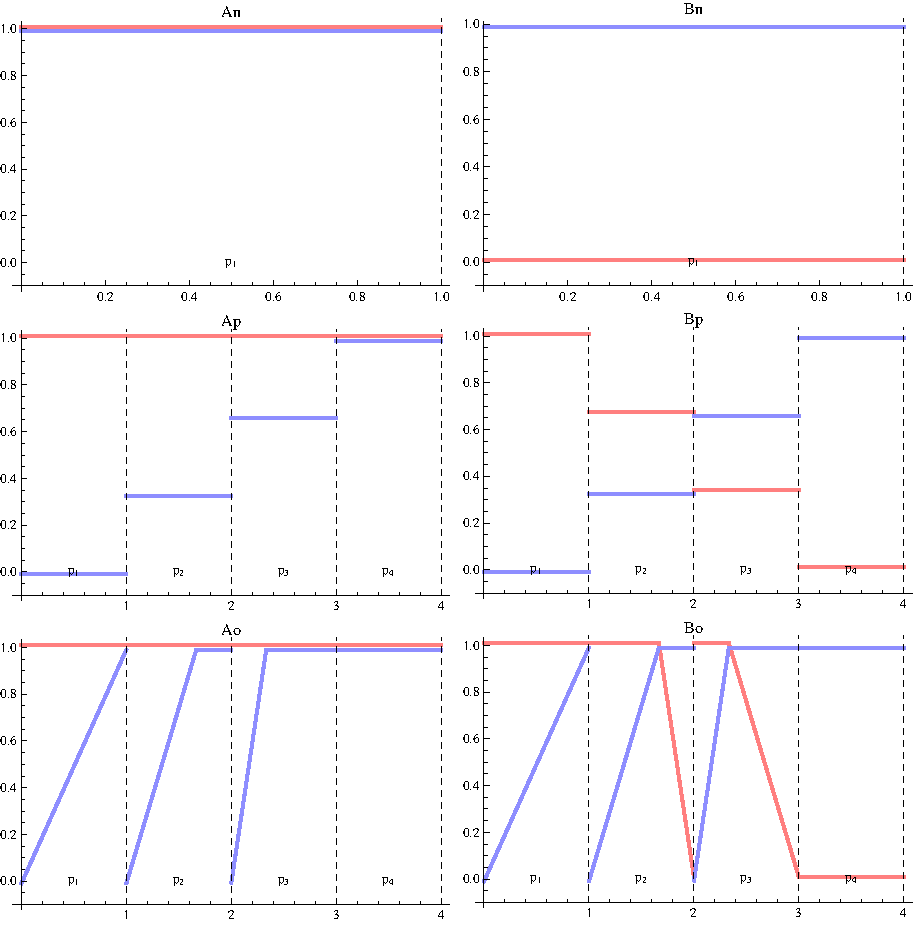
\includegraphics[scale=1.0]{fig/morph-regiment.pdf} 
  \vspace{-15pt}
  \caption[Variations of morphological
    change]{\label{morph-regiment}An, Bn do not change morphology;
    Ap, Bp change morphology over phylogenetic time; Ao, Bo change
    morphology over ontogenetic and phylogenetic time.}
\end{figure}
\end{comment}

\begin{figure}
  \centering
  \figtitle{Variations of Morphological Change for $A$} 
  \hspace*{-30pt} 
  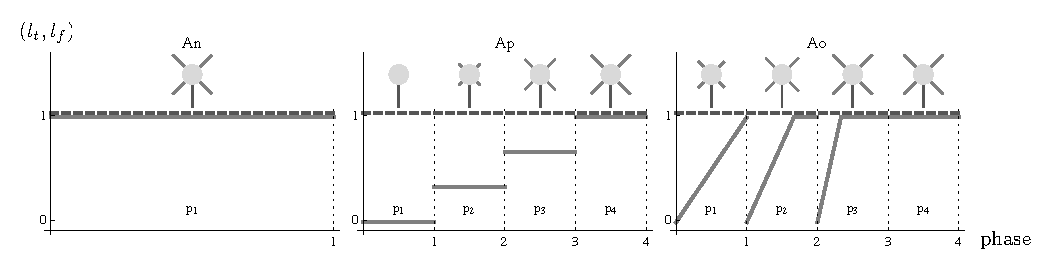
\includegraphics[scale=1.0]{fig/morph-var-a.pdf} 
  \vspace{-15pt}
  \caption[Variations of morphological change]{\label{fig:morph-var-a}
    Shows how the morphology is controlled for each phase $p_i$ for
    adult forms $A$ where the infant form is conserved.  An
    does not change its morphology; Ap changes its morphology over
    phylogenetic time; Ao changes its morphology over ontogenetic and
    phylogenetic time.}
\end{figure}

\begin{figure}
  \centering
  \figtitle{Variations of Morphological Change for $B$} 
  \hspace*{-30pt} 
  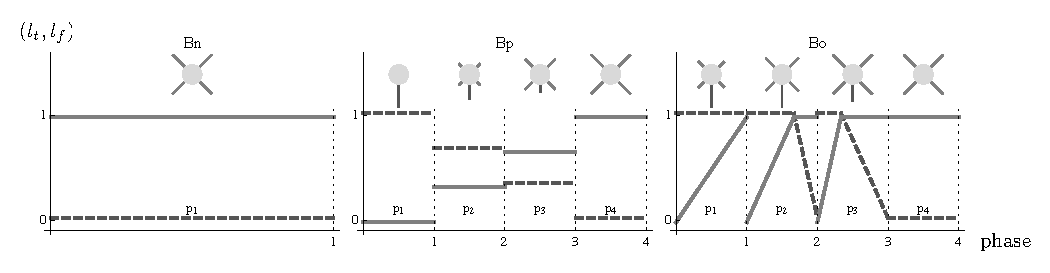
\includegraphics[scale=1.0]{fig/morph-var-b.pdf} 
  \vspace{-15pt}
  \caption[Variations of morphological change]{\label{fig:morph-var-b}
    Shows how the morphology is controlled for each phase $p_i$ for
    adult forms $B$ where the infant form is not conserved.  Bn does not
    change its morphology; Bp changes its morphology over phylogenetic
    time; Bo changes its morphology over ontogenetic and phylogenetic
    time.}
\end{figure}



\section{Controller Variation}

In the test cases $Bp$ and $Bo$ the infant form is not conserved in
the adult form.  However, the controller may conserve some behaviour
acquired in the infant form that is useful in the adult form, which
may accelerate evolution.  To determine whether this happens, two
types of CTRNN controllers are considered: 1) a ``lobotomised''
controller, which has two independent CTRNNs, one for the tail; one
for the feet. 2) a ``non-lobotomised'' controller, which has one CTRNN
that controls both the tail and feet.  These are shown in
Figure~\ref{ctrnn-figures}.

\begin{figure}[h]
  \centering
  \figtitle{Variation of CTRNN Controllers} 
  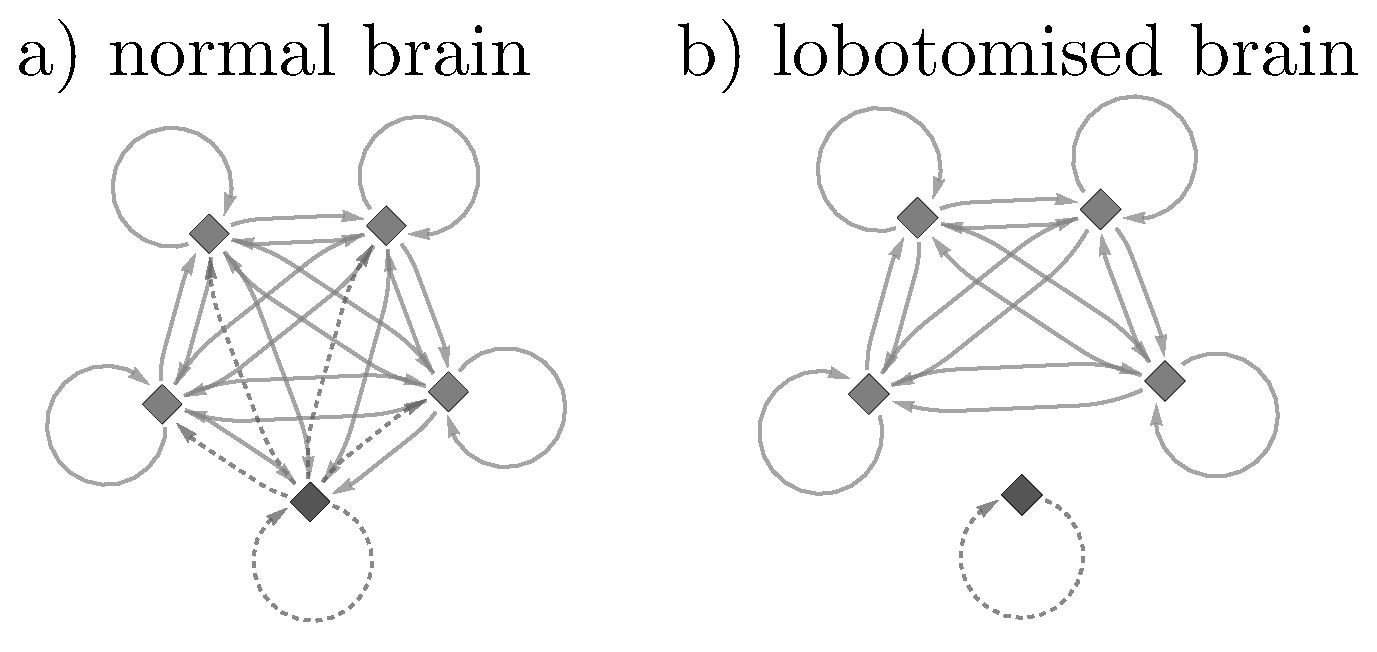
\includegraphics[width=5in]{fig/ctrnn-figures-gs.pdf} 
  \vspace{-15pt}
  \caption[Variation of CTRNN controllers]{\label{ctrnn-figures}a)
    Fully connected CTRNN controller. b) Independent CTRNN controllers
    for the tail and legs.  The dashed lines represent the connections
    from the tail and to the motor neuron for the tail.  The solid
    lines represent connections from or to a motor neuron for a
    foot. }
\end{figure}

The sensors are altered for the ``lobotomised'' controller.  The tail
brain does not receive proprioceptive sensors from the other limbs
$\{s_7, s_8, \ldots, s_{14}\}$.  Likewise, the foot brain does not
receive proprioceptive sensors from the tail $s_5$ and $s_6$.
Otherwise, the sensors are the same.\footnote{Note on implementation:
  the ``lobotomised'' controller code is the same as the
  ``non-lobotomised'' with a specific set of weights $w_{ji}$ and
  sensor coefficients $n_{ji}$ set to zero.}

\section{Tasks}

To confirm the results are not spurious or a special case for one
particular task, multiple tasks of varying difficulty are considered.
The basic task is locomotion to a target.  Changing the target
location was considered, but it is hard to ascertain what positions of
the target would be more difficult.  The infant ``tadpole'' form with
its tail directed to the south and a target to the west have to turn
before it could locomote toward the target, so it may be more
difficult for the infant form.  However, the adult ``frog'' form is
symmetric with respect to targets placed in the cardinal directions,
so there is no discernable difference in difficulty.  Changing the
position of the target does not provide a simple means of constructing
more difficult tasks.  

\begin{comment}
Bongard's work has a task that is simpler for the infant than for the adult
\end{comment}

Instead of changing the target location, varying the velocity of
current $\bv v_c$ is considered.  Each individual is affected
similarly by the current--regardless of its morphology.\footnote{This
  differs from Bongard's work where the task was easier for the infant
  form due to its morphology.}  In task 1 the current assists the
individual to the target.  In task 2 there is no current.  In task 3
the current pulls the individual laterally away from the target.  In
task 4 the current is directly against the
target. Figure~\ref{fig:tasks} shows a diagram of the tasks.  The
tasks are meant to be in an ascending order of
difficulty.\footnote{One could argue that the task 1 may in fact be
  more difficult because it may require two skills: go and stop.}

\begin{figure}
  \centering
  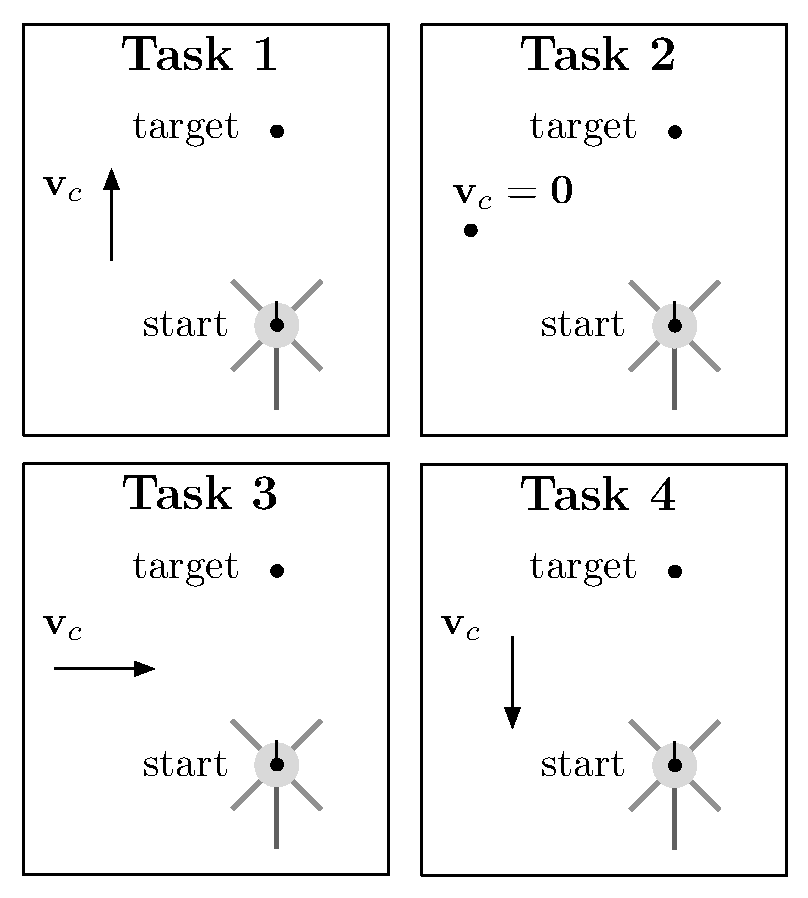
\includegraphics[scale=0.8]{fig/tasks.pdf} 
  \caption[Tasks]{\label{fig:tasks}Tasks shown in an ascending order
    of difficulty.}
\end{figure} 

\section{Evolutionary Algorithm}

The evolutionary algorithm used is described in detail in
\cite{Bongard:2011p3556}.  The algorithm is a variant of the steady
state Age-Layered Population Structure (ALPS)
\cite{Hornby:2009p3558,Hornby:2006p3649}.  The population is divided
into layers based on the age of the individuals.  The bottom layer
holds the youngest individuals and is periodically reset with new
genetic material.  The top layer holds the oldest individuals.  By
segregating individuals based on age, ALPS maintains population
diversity and avoids premature convergence to local
optima\cite{Hornby:2006p3649}.

\begin{comment}
The age of an individual $i$ is defined as $a_i = \lfloor
\frac{n}{N(pop)} \rfloor$ where $n$ is the optimisation step and
$N(pop)$ is the population size.
\end{comment}

Each individual has an age and each layer has an age limit.  An
individual whose age is greater than this age limit is defined to be
too old.  It may dislodge another individual $j$ in the next layer if
its fitness $\bv f_i$ dominates $\bv f_j$\footnote{Note: in this case
  lower values for fitness are considered better.}.  If it cannot
dislodge any individuals, it is discarded.

\begin{eqnarray}
  \bv a \text{ dominates } \bv b \iff a_i < b_i ~ \forall i
\end{eqnarray}

An individual is dominated if any other individual in its layer
dominates it.  In this ALPS variant, only non-dominated individuals
within the layer are allowed to reproduce.  Reproduction happens as
follows: A copy of the parent is made.  Each element of its genome has
a $0.05$ chance of being reset to a random uniform value in the
interval $[0, 1]$.  No crossover operation is used.

\begin{comment}


  big conclusions:
   - tasks need not be easier because of morphology (if it works)
   - simpler controllers can accelerate evolution
     - hmm, I could switch between an oscillator and a CTRNN
     - maybe even if nothing is conserved between the infant and adult form
\end{comment}

\chapter{Results}

A run can be described by three pieces of information: The
morphological variation $\{An, Bn, Ap, Bp, Ao, Bo\}$, the task
$\{1,2,3\}$, and whether it is lobotomised $\{0, 1\}$.  A trial is
usually comprised of 6 runs--one for each morphological variation--and
it is described by the task and lobotomised state.

\section{Results for Task 1}

Figure~\ref{fig:evals-t1-l0} shows the results for task 1.
Statiscally significant differences were found; however, the
differences indicate that it takes longer for evolution to find a
solution when the morphology changes phenogenetically or
ontogenetically, which may be a reasonable expectation since one is
asking for the optimisation procedure to effectively solve multiple
problems in succession instead of one problem.  One of the aims of
this work was to produce results similar to those found in
\cite{Bongard:2011p3716}, and attempt to draw clearer boundaries
between what kind of morphological change can accelerate evolution.
Still it may be instructive to determine where all the evaluations
were spent.

\begin{figure}
  \centering
  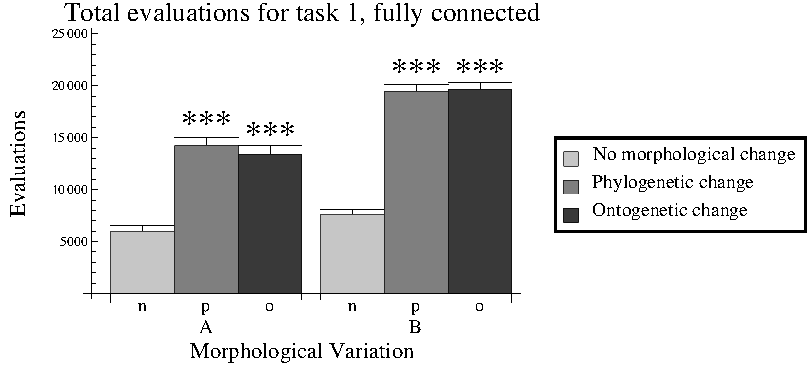
\includegraphics[scale=1]{fig/evals-t1-l0.pdf} 
  \caption[Total evaluations for task 1, fully
    connected]{\label{fig:evals-t1-l0}This chart shows the mean number
    of evaluations over 100 independent trials (100 * 6 runs) for each
    of the morphological variations on task 1 with a fully connected
    controller.  The bar represents the standard error.  The stars
    indicate whether the difference in mean (e.g., $Ap$, $Ao$) is a
    statistically significant compared to the control (e.g., $An$)
    according to a Mann--Whitney U test.  }
\end{figure}

Figure~\ref{fig:step-evals-t1-l0} shows the mean number of evaluations
per phase for the same set of results shown in
Figure~\ref{fig:evals-t1-l0}.  Phase 1 and 2 both complete well before
the only phase in $An$ and $Bn$, the baseline each are compared
against.  Phase 3, however, takes a majority of the evaluations for
most of the morphological variations.  Why is that?  Examining the
most extreme case $Bp$ may be instructive.

\begin{figure}
  \centering
  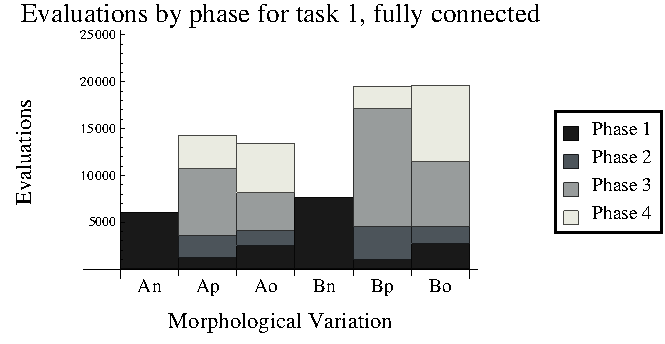
\includegraphics[scale=1]{fig/step-evals-t1-l0.pdf} 
  \caption[Evaluations by phase for task 1, fully
    connected]{\label{fig:step-evals-t1-l0}This chart shows the mean
    number of evaluations per phase over 100 independent trials (100 *
    6 runs) for each of the morphological variations on task 1 with a
    fully connected controller.  }
\end{figure}


Figure~\ref{fig:morph-var-b} shows that phase 3 of $Bp$ changes both
the tail $l_t$ and the feet $l_f$, essentially swaping the values.
Perhaps the transition from the tail being the main source of
locomotive power to the feet is the cause.  It could be that altering
both variables simultaneously is not conducive to the kind of
scaffolding that may be required to exhibit an acceleration of
evolution.  That would be supported by examining phase 3 of $Ap$ which
only alters the foot length $l_f$ and does not require as many
evaluations.

One further curiosity to note about figure~\ref{fig:step-evals-t1-l0}
is that phase 4 for $Ao$ and $Bo$ both require a fair amount of
evaluations for what looks like a comparatively small change
morphologically.  For the $Bo$ case, phase 4 appears to take as long
as $Bn$ which suggests that the preceding phases have not accelerated
evolution at all.  In fact, performing a Mann--Whitney U test on the
two sets of data reveals they do not statistically differ ($p =
0.74$).  Therefore, the morphological variation $Bo$ represents a case
where the conditions assuredly do not accelerate evolution.

Phase 4 of $Bo$ can be instructive in trying to determine what
conditions are necessary.  Further more, it suggests a good experiment
to determine whether any acceleration is happening: run each phase
independent of the others with a random population and compare mean
evaluations.  $Bn$ and phase 4 of $Bo$ are just such a case and can be
compared directly.  In fact, the last phase of all the morphological
variations are comparable in this way. The other cases do
statistically differ according to the Mann--Whitney U test despite
phase 4 of $Ao$ looking potentially close to $An$ ($p = 3.0 \times
10^{-4}$).

Examining phase 4 of $Ap$ and $Bp$ in isolation demonstrates two cases
where the populations are primed to succeed by the preceeding phases.
Granted the preceeding phases, especially phase 3, have made those
gains not worthwhile commulatively, but they may be instructive yet.
One oddity is comparing $Ap$ which only alters $l_f$ and $Bp$ which
alters both $l_f$ and $l_t$ yet $Bp$ takes less time than $Ap$ ($p =
8.1 \times 10^{-3}$), so the simultaneous changing of variables need
not cause automatic concern.

\section{Results for Task 2}

Task 2 was run similarly to task 1 with the exception that fewer
trails were conducted.  The reason being that because the magnitudes
were so different between the control and the experimental group, it
does not require many runs to determine a statistical difference in
the distributions.  

The results for task 2 do not look dramatically different from task 1.
One gratifying aspect is that task 2 does appear to be more difficult
than task 1 as intended.  The median evaluations for $An$ task 1 and 2
are 4562.5 and 6495; the distributions differ (Mann-Whitney U $=1122$,
$n_1 = 100$, $n_2 = 32$, $\mu_1 < \mu_2$, $p = 0.0055 < 0.01$).

\begin{figure}
  \centering
  \includegraphics[scale=1]{fig/evals-t2-l0.pdf} 
  \caption[Total evaluations for task 2, fully
    connected]{\label{fig:evals-t2-l0}This chart shows the mean number
    of evaluations over 32 independent trials (32 * 6 runs) for each
    of the morphological variations on task 2 with a fully connected
    controller.  The bar represents the standard error.  The stars
    indicate whether the difference in mean between the experimental
    (e.g., $Ap$, $Ao$) is a statistically significant compared to the
    control (e.g., $An$) according to a Mann--Whitney U test.  }
\end{figure}

\begin{figure}
  \centering
  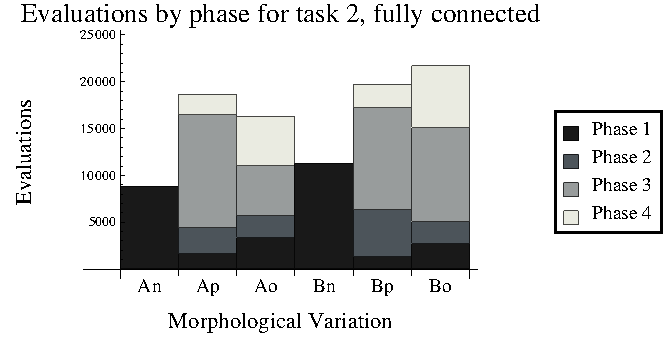
\includegraphics[scale=1]{fig/step-evals-t2-l0.pdf} 
  \caption[Evaluations by phase for task 2, fully
    connected]{\label{fig:step-evals-t2-l0}This chart shows the mean
    number of evaluations per phase over 32 independent trials (32 * 6
    runs) for each of the morphological variations on task 1 with a
    fully connected controller.  }
\end{figure}
